
\subsection{Popis GUI} \label{popis-gui}
V této kapitole se budeme zabývat za jakých okolností se spustí jaké obrazovky.

% Stavy vzhledem ke GUI.
Nejprve specifikujeme v jakých stavech se STM může nacházet.
Toto jsou pouze stavy, které nás zajímavý v kontextu GUI - tj. v kontextu toho co všechno chceme
uživateli zobrazit.
Rozhodně se nejedná o souhrn všech možný stavů.
\subsubsection{Stavy STM}
\begin{itemize}
  \item Ethernetová periferie je korektně inicializována a kabel je připojen. Zkráceně budeme
        značit \texttt{ETH-up}.
  \item Ethernetový kabel je buď odpojen nebo Ethernetová periferie se z nějakého důvodu
        neinicializovala. Zkráceně budeme značit jako \texttt{ETH-down}.
  \item STM je připojeno k serveru. Zkráceně značíme \texttt{CONNECTED}.
  \item STM je odpojeno od serveru. Zkráceně značíme \texttt{DISCONNECTED}.
  \item STM se připojuje k serveru, s tím že je nastavený (TODO) nějaký timeout. Zkráceně značíme
        \texttt{CONNECTING}.
  \item V EEPROM nejsou uložena žádná konfigurační data intervalů. Tento stav nastává pouze v případě,
        kdy uživatel zapne STM poprvé.
  \item V EEPROM jsou uložena konfigurační data intervalů.
  \item Uživatel už zadal klíč (viz ...) do STM. Tento klíč se ukládá do EEPROM, aby ho uživatel
        nemusel zadávat opakovaně.
  \item Uživatel ještě klíč nezadal. To znamená, že se ještě nepokoušel připojit k serveru.
\end{itemize}

% Invarianty - co chceme aby v rámci GUI platilo.
\subsubsection{Invarianty}
ETH-up a ETH-down se může v podstatě libovolně střídat v běhu aplikace a chceme o tom uživateli
dát vědět.
Pokud se za běhu aplikaceme dostaneme do stavu \texttt{ETH-up}, dáme uživateli možnost připojit
se k serveru.
Pokud jsme ve stavu \texttt{CONNECTED}, nemůžeme se odpojit. Jedině pokud resetujeme celé STM.
Pokud STM vůbec není připojeno k internetu a EEPROM je prázdná, dáme uživateli možnost nastavit
intervaly.

% Popis přepínání mezi obrazovkami
\subsubsection{Popis jednotlivých obrazovek}

% Vyjmenování GUI prvků, které budeme potřebovat
V rámci celého GUI nám stačí tyto grafické prvky:
\begin{itemize}
  \item Tlačítka, pomocí kterých budeme chtít potvrzovat data zadaná do jednotlivých obrazovek
    a přepínat tím na další obrazovky.
  \item Okna s nastavitelnou hodnotou kde hodnota může být například čas v minutách, nebo teplota.
    Uživatel může hodnotu nastavit pomocí joysticku.
  \item Okna, která slouží pouze pro zobrazování nějaké hodnoty - například aktuálního času, nebo
    naměřené teploty.
  \item Různé nápisy resp. nadpisy pro lepší přehlednost.
\end{itemize}

Nejprve uvedeme nákresy jednotlivých obrazovek a popíšeme co znamenají.
Potom uvedeme tzv. frame diagram tj. stavový diagram obrazovek, kde popíšeme jak se mezi sebou
jednotlivé obrazovky přepínají.

Zeleně zabarvený text v obrázcích (TODO: ztučněný, pokud nebudeme tisknout barevně) představuje
buď nakliknutelný čudlík nebo měnitelný prvek - například čas.
Jak jsme již zmiňovali STM se ovládá pomocí joysticku pod displejem.
Pohybem joysticku do stran přepínáme mezi jednotlivými nakliknutelnými prvky.
Pohybem joysticku nahoru a dolu měníme hodnoty právě nakliknutých prvků, pokud to jde.
Nakliknutý prvek na displeji STM poznáme podle červeného zabarvení.

% ClkFrame
\paragraph{ClkFrame}
% TODO: footnote - názvy jednotlivých obrazovek odpovídají názvům tříd, které jsou zmíněné v kapitole
%   architektura.
\begin{figure}[H]\centering
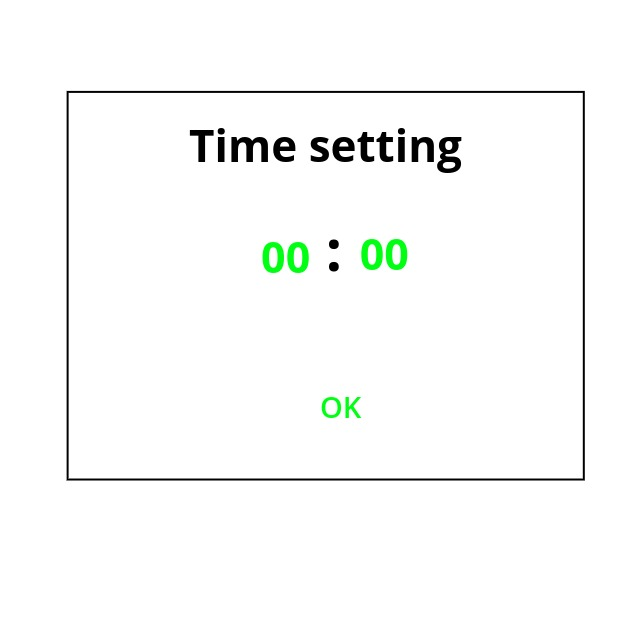
\includegraphics[width=140mm, height=140mm]{../img/clk_frame.jpg}
\caption{ClkFrame - nastavení času}
\label{clk-frame}
\end{figure}

Tato obrazovka je zobrazena po startu STM v momentě, kdy Ethernetová periferie není inicializována a
STM se tedy nemůže připojit k serveru aby rovnou synchronizovalo čas.

% SetIntervalFrame
\paragraph{SetIntervalFrame}
\begin{figure}[H]\centering
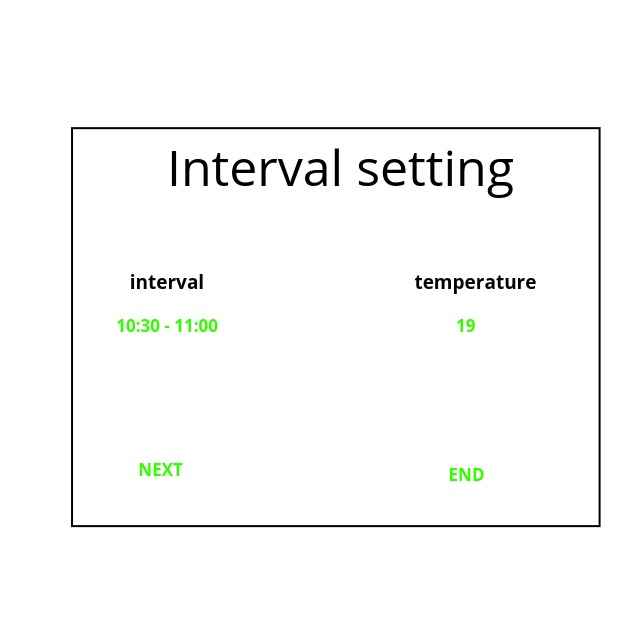
\includegraphics[width=140mm, height=140mm]{../img/interval_setting_frame.jpg}
\caption{SetIntervalFrame - nastavení intervalů}
\label{set-interval-frame}
\end{figure}

Tato obrazovka umožňuje uživateli nastavit časové intervaly s teplotou.
Obrazovka zobrazuje nastavení pro právě jeden interval, pokud uživatel stiskne tlačítko
"Next", zobrazí se nastavení dalšího intervalu, pokud stiskne tlačítko "End", nastavování
intervalů se ukončí a všechny nastavené intervaly jsou uloženy do EEPROM.

Zobrazena je v těchto případech:
\begin{itemize}
  \item když EEPROM neobsahuje žádné nastavení intervalů což nastává v případě kdy uživatel
    ještě žádné intervaly nenastavoval - tedy po prvním spuštění STM.
  \item Když uživatel zmáčkne v obrazovce \texttt{MainFrame} čudlík "reset intervals".
\end{itemize}

% OverviewIntervalFrame
\paragraph{OverviewIntervalFrame}
OverviewIntervalFrame neboli "přehled všech nastavených intervalů" vypadá stejně jako SetIntervalFrame
až na to, že intervaly nejdou nastavovat, pouze prohlížet.
Tlačítkem "Next" se můžeme proklikat postupně přes všechny intervaly a tlačítkem "End" zobrazování
ukončit.

% ConnectFrame
\paragraph{ConnectFrame}
\begin{figure}[H]\centering
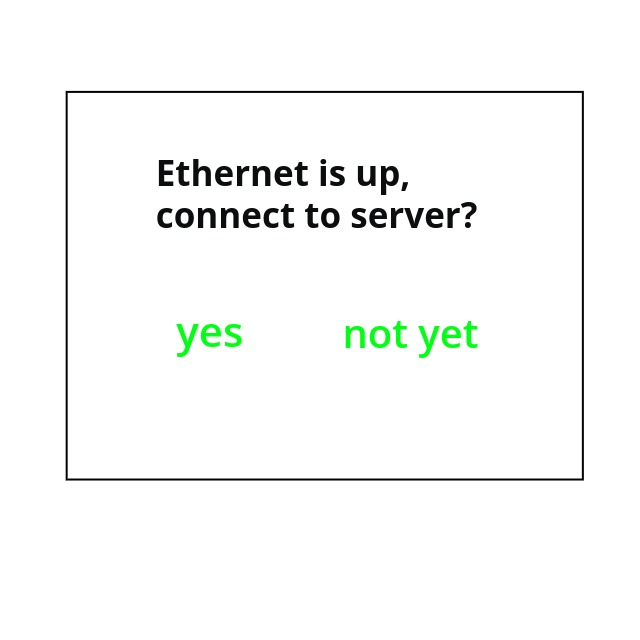
\includegraphics[width=140mm, height=140mm]{../img/connect_frame.jpg}
\caption{ConnectFrame - připojení k serveru}
\label{connect-frame}
\end{figure}

Tato obrazovka je zobrazena ihned po spuštění STM v momentě, kdy Ethernetová periferie je inicializována
a klíč ještě není uložen v EEPROM.
V takovém případě se STM může ihned připojit k serveru a nemusíme uživatele zdržovat s nastavováním
času.

% KeyFrame
\paragraph{KeyFrame}
\begin{figure}[H]\centering
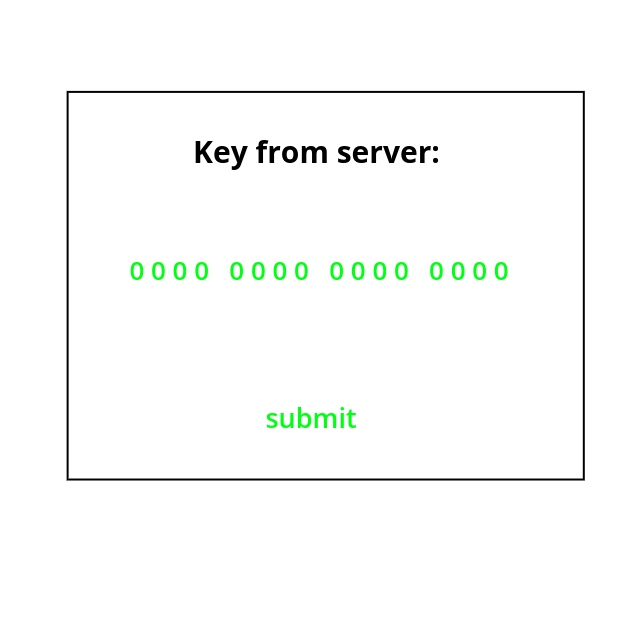
\includegraphics[width=140mm, height=140mm]{../img/key_frame.jpg}
\caption{KeyFrame - zadání klíče vygenerovaného serverem}
\label{key-frame}
\end{figure}

Do této obrazovky uživatel musí zadat 8-bytový DES klíč vygenerovaný na serveru.
Po stisknutí tlačítka "Submit" se STM pokusí přihlásit na server.

% MainFrame
\paragraph{MainFrame}
\begin{figure}[H]\centering
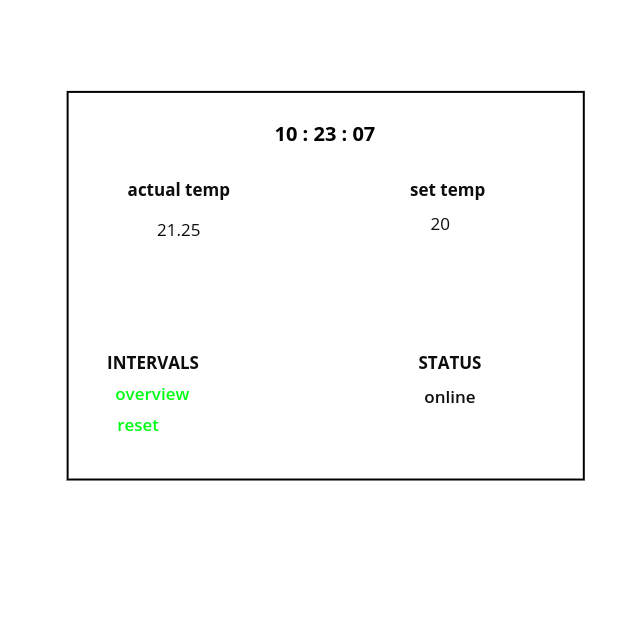
\includegraphics[width=140mm, height=140mm]{..//img/main_frame_online.jpg}
\caption{MainFrame - hlavní obrazovka}
\label{main-frame}
\end{figure}

MainFrame reprezentuje hlavní obrazovku.
Jsou zde zobrazeny zásadní hodnoty - aktuálně naměřená teplota (actual temp), přednastavená teplota
(set temp), stav připojení k serveru.
% tlačítko connect
Pokud je stav \texttt{DISCONNECTED} a zároveň \texttt{ETH-up}, objeví se v MainFrame tlačítko "connect",
pomocí kterého se uživatel dostane na obrazovku KeyFrame, kam může zadat klíč vygenerovaný serverem a
připojit se tak na server.
V případě kdy je klíč uložen v EEPROM, tak se STM, po stisku tlačítka "connect" rovnou připojí k serveru
a pouze zobrazí stav \texttt{CONNECTING}.

Uživatel se z MainFrame také může dostat do SetIntervalFrame pomocí "reset intervals" tlačítka a do
OverviewIntervalFrame pomocí "overview intervals" tlačítka.

%%%%%%%%%%%%%%%
% Frame diagram
%%%%%%%%%%%%%%%
\subsubsection{Vztahy mezi obrazovkami}

\begin{figure}[H]\centering
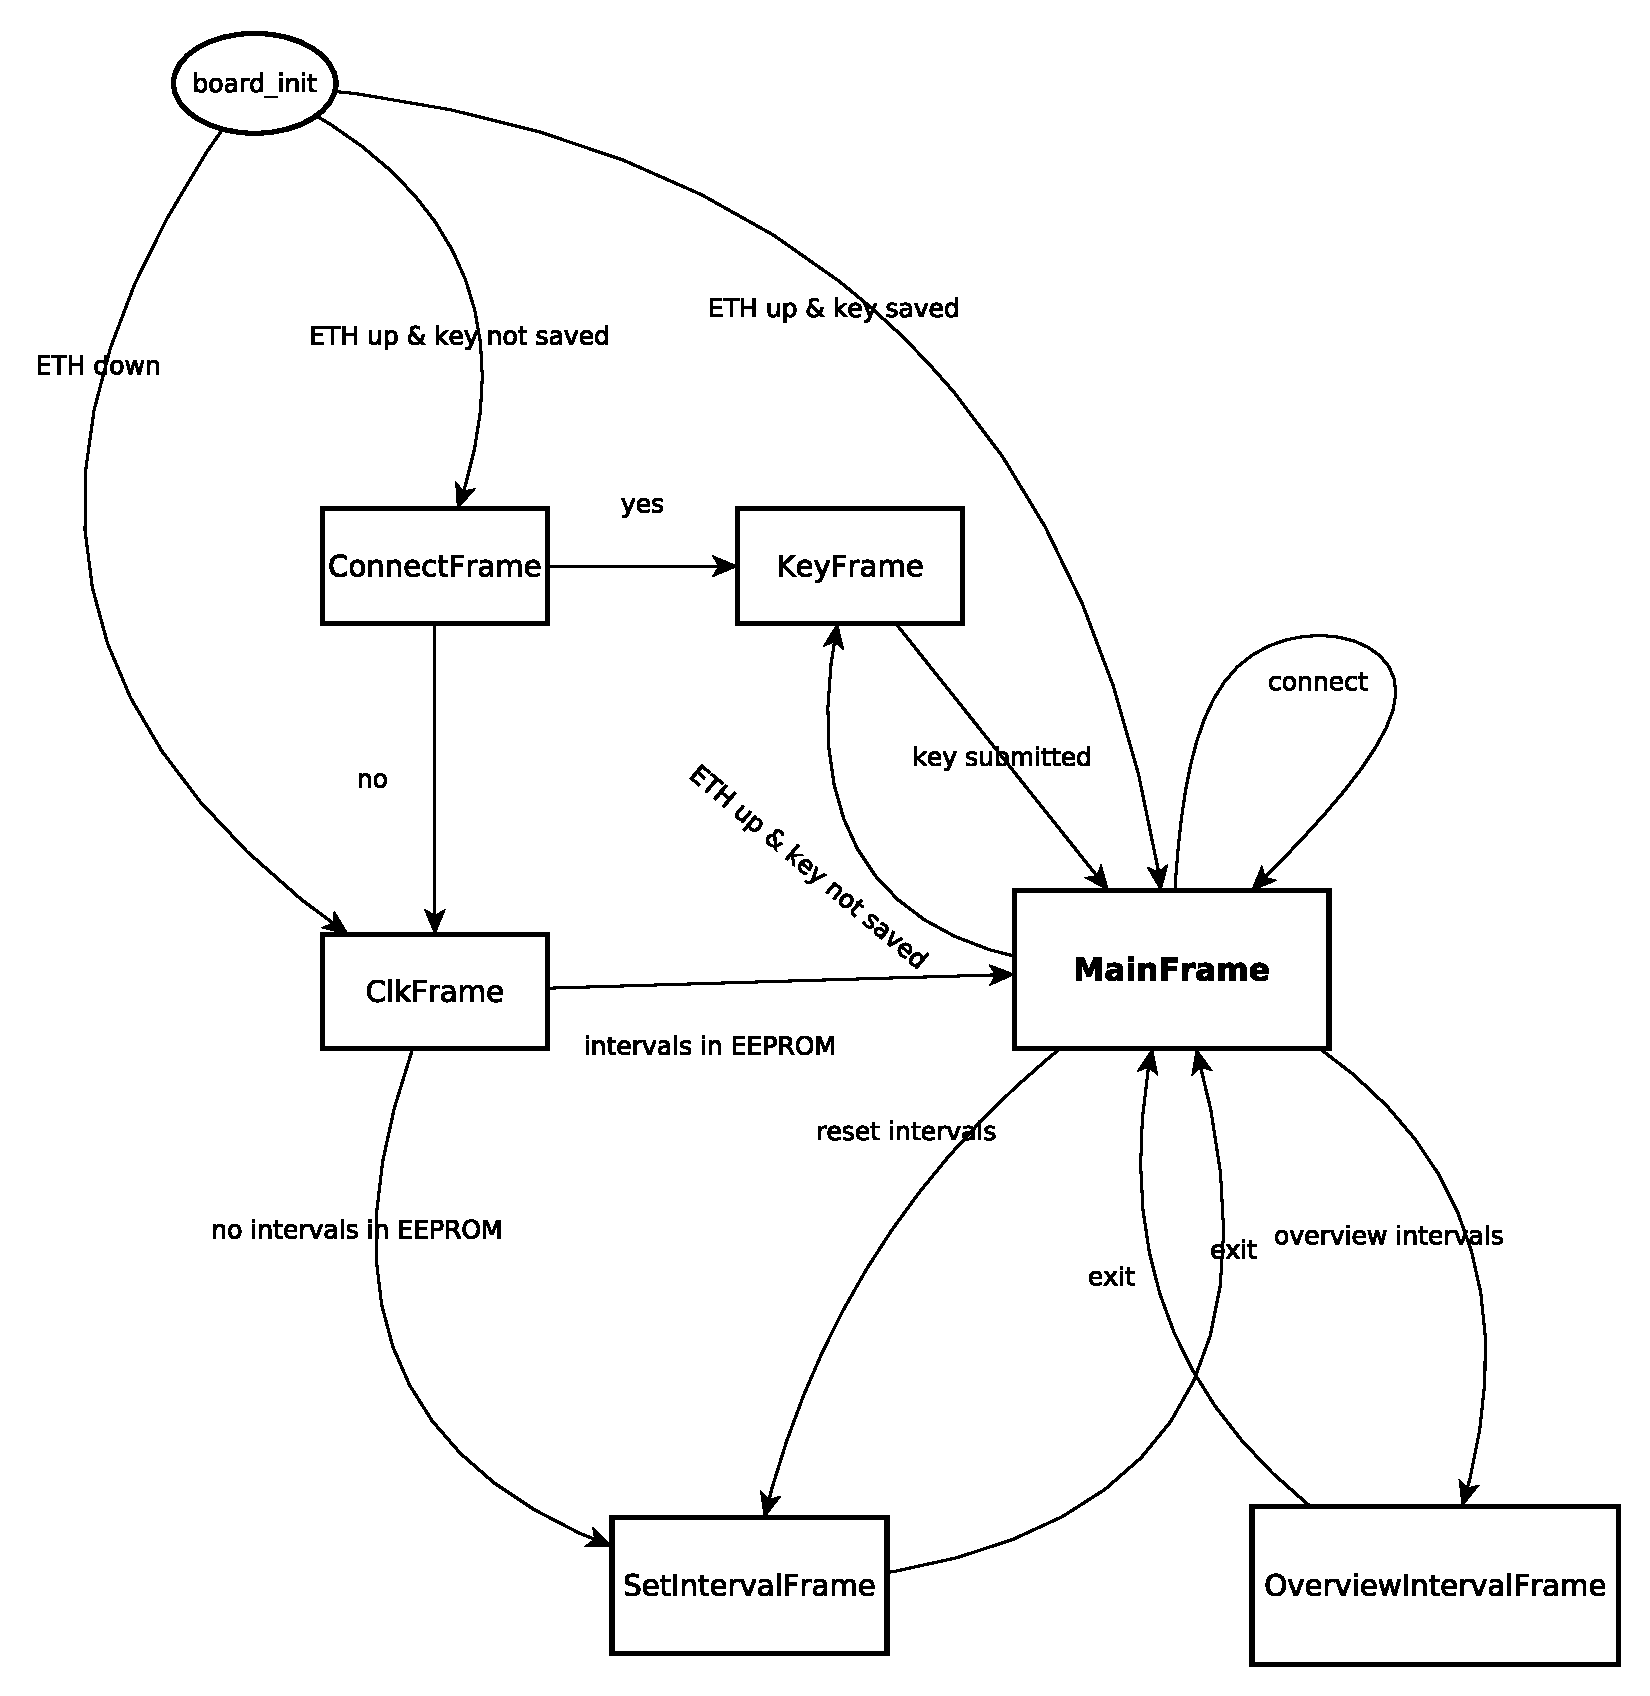
\includegraphics[width=140mm, height=140mm]{../diagrams/frame_diagram.pdf}
\caption{Diagram přepínání obrazovek}
\label{frame-diagram}
\end{figure}

